% !TEX root = ../main.tex

% Ruimin Huang
\begin{IEEEbiography}[{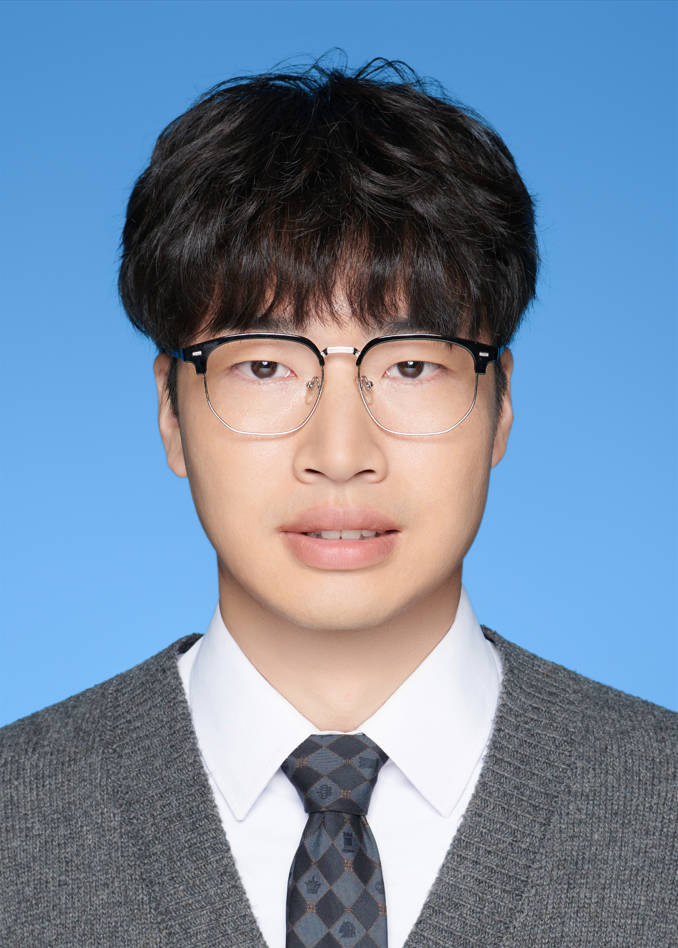
\includegraphics[width=1.1in,height=1.35in,clip,keepaspectratio]{./figs/biography/Ruimin_Huang}}]{Ruimin Huang} received the M.S. degree in optical engineering from the School of Physics and Electronic Information, Yunnan Normal University, Kunming, China, in 2024. He is currently pursuing the Ph.D. degree in electronic information with the Electronic Information School, Wuhan University, Wuhan, China.

His research interests include computer vision, infrared technology, and remote sensing.
\end{IEEEbiography}

% Jun Huang
\begin{IEEEbiography}[{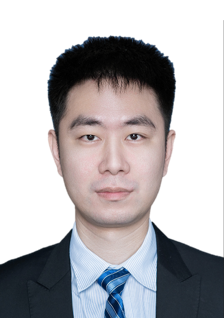
\includegraphics[width=1.1in,height=1.35in,clip,keepaspectratio]{./figs/biography/Jun_Huang}}]{Jun Huang} (Member, IEEE) received the B.S. degree in communication engineering and the Ph.D. degree in electronic circuit and system from the Huazhong University of Science and Technology, Wuhan, China, in 2008 and 2014, respectively.

He is currently a Professor with the School of Robotics, Wuhan University, Wuhan. His main research interests include infrared image and infrared spectrum processing.
\end{IEEEbiography}

% Yong Ma
\begin{IEEEbiography}[{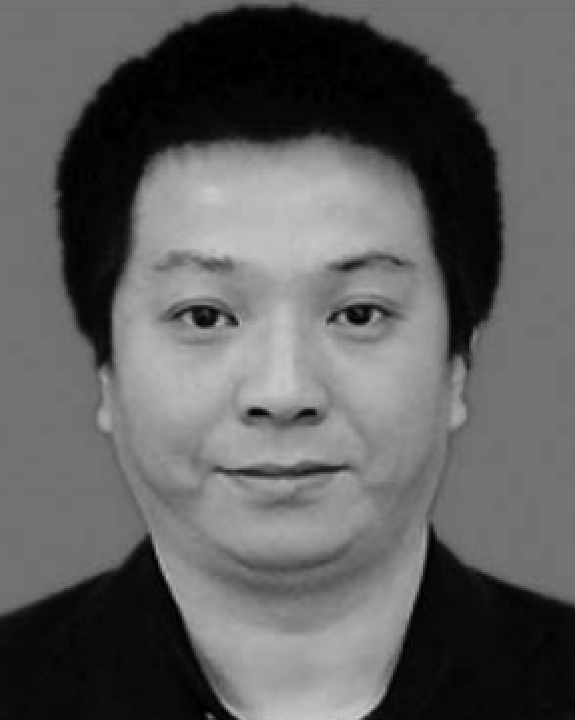
\includegraphics[width=1.0in,height=1.34in,clip,keepaspectratio]{./figs/biography/Yong_Ma}}]{Yong Ma} received the B.S. degree in industrial automation and the M.S. degree in automatic control from the Beijing Institute of Technology, Beijing, China, in 1994 and 1997, respectively, and the Ph.D. degree in electronic circuit and system from the Huazhong University of Science and Technology (HUST), Wuhan, China, in 2003.

From 2004 to 2006, he was a Lecturer with the University of the West of England, Bristol, U.K. From 2006 to 2014, he was a Professor of electronics with Wuhan National Laboratory for Optoelectronics, HUST. He is currently a Professor with the School of Robotics, Wuhan University, Wuhan. His research interests include signal and systems, infrared image processing, pattern recognition, and interface circuits to sensors and actuators.
\end{IEEEbiography}

% Fan Fan
\begin{IEEEbiography}[{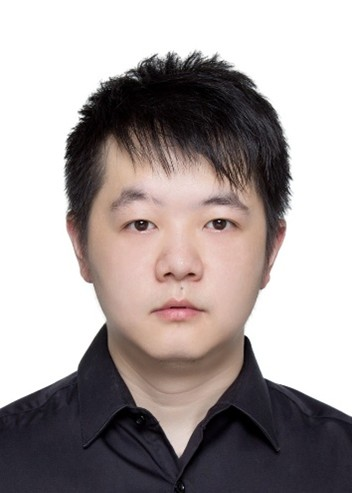
\includegraphics[width=1.1in,height=1.35in,clip,keepaspectratio]{./figs/biography/Fan_Fan}}]{Fan Fan} (Member, IEEE) received the B.S. degree in communication engineering and the Ph.D. degree in electronic circuit and system from the Huazhong University of Science and Technology, Wuhan, China, in 2009 and 2015, respectively.

He is currently an Associate Professor with the School of Robotics, Wuhan University, Wuhan. His research interests include infrared thermal imaging, machine learning, and computer vision.
\end{IEEEbiography}

% Yiming Zhu
\begin{IEEEbiography}[{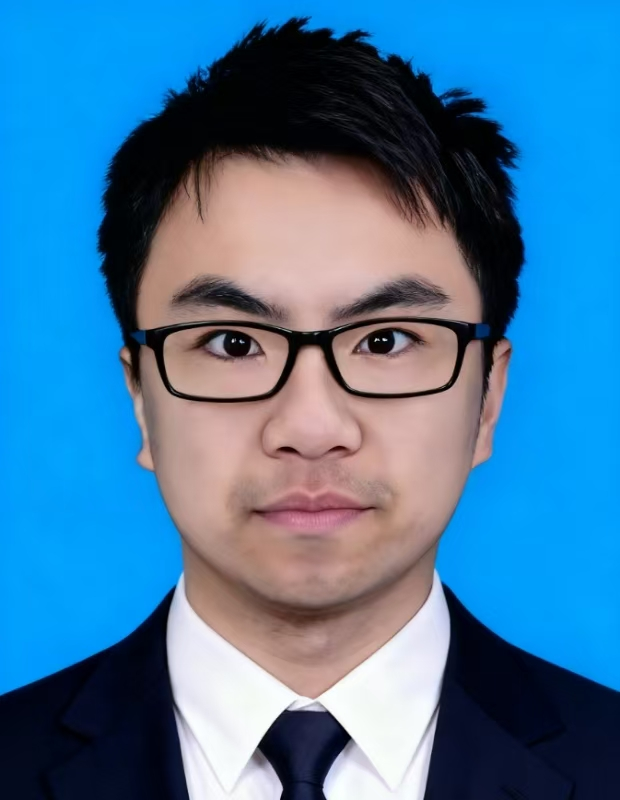
\includegraphics[width=1.0in,height=1.35in,clip,keepaspectratio]{./figs/biography/Yiming_Zhu}}]{Yiming Zhu} received the M.S. degree in optical engineering from the School of Optics and Photonics, Beijing Institute of Technology (BIT), Beijing, China, in 2022. He is currently pursuing the Ph.D. degree with the Multi-Spectral Vision Processing (MVP) Lab, Electronic Information School, Wuhan University, Wuhan, China.

His research interests include computer vision, infrared technology, and remote sensing.
\end{IEEEbiography}
